\chapter{Estado del Arte}

Con el propósito de caracterizar el estado actual de la investigación sobre modelos probabilísticos aplicados a la detección de Amenazas Persistentes Avanzadas, esta sección presenta la síntesis y el análisis de los estudios seleccionados mediante el proceso de revisión sistemática descrito previamente. El análisis se estructura en función de las preguntas de investigación definidas, lo que permite examinar los enfoques empleados, los conjuntos de datos utilizados y las estrategias adoptadas frente al desbalance de clases. A partir de la evidencia recopilada se identifican tendencias, fortalezas y limitaciones de las soluciones existentes, así como las brechas que fundamentan la propuesta presentada en este trabajo.

\section{Panorama bibliométrico del corpus}

El corpus final quedó constituido por 77 estudios primarios, de los cuales 70 corresponden a artículos de revista y 7 a comunicaciones en conferencias. La revista IEEE Access concentra la mayor proporción de publicaciones del corpus, con 17 estudios, seguida por IEEE Transactions on Dependable and Secure Computing.

La distribución temporal, presentada en la Figura~\ref{fig:temporal}, evidencia un crecimiento sostenido del interés investigativo en el área. Mientras que entre 2017 y 2022 la producción se mantuvo en un rango de tres a ocho estudios anuales, a partir de 2023 se observa una expansión marcada, que alcanza 22 estudios en 2026. Más de la mitad del corpus corresponde a publicaciones de los últimos tres años, lo que confirma que se trata de un área de investigación activa y en desarrollo, y no de un campo consolidado con soluciones establecidas.

\begin{figure}[h!]
\centering
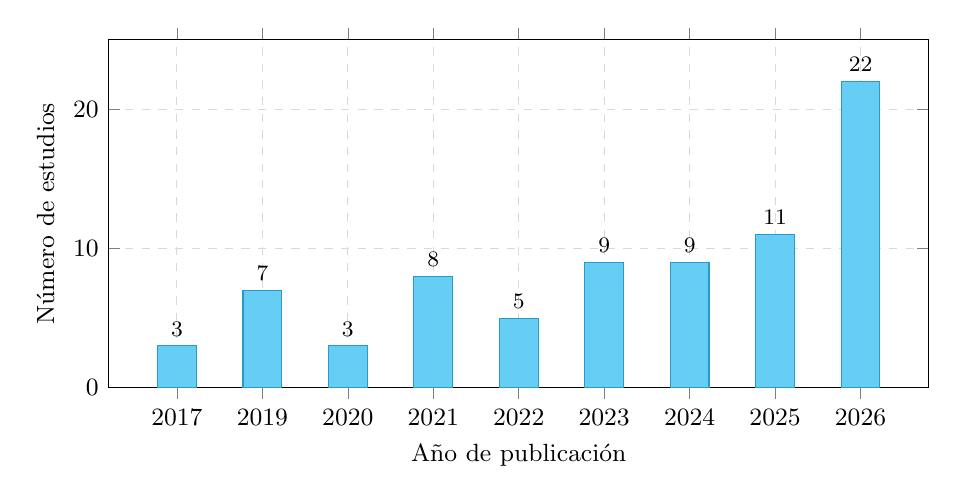
\begin{tikzpicture}
\begin{axis}[
    width=12cm, height=6cm,
    ybar, bar width=14pt,
    ymin=0, ymax=25,
    symbolic x coords={2017,2019,2020,2021,2022,2023,2024,2025,2026},
    xtick=data,
    ylabel={Número de estudios},
    xlabel={Año de publicación},
    nodes near coords, nodes near coords style={font=\footnotesize},
    grid=major, grid style={dashed,gray!30},
    tick label style={font=\small}, label style={font=\small},
]
\addplot[fill=cyan!60,draw=cyan!80!black] coordinates {(2017,3)(2019,7)(2020,3)(2021,8)(2022,5)(2023,9)(2024,9)(2025,11)(2026,22)};
\end{axis}
\end{tikzpicture}
\caption{Distribución temporal de los estudios del corpus (2017--2026). Fuente: Elaboración propia.}
\label{fig:temporal}
\end{figure}

La Figura~\ref{fig:modelos} presenta la distribución de los estudios según la familia de modelos que mencionan en su texto completo, conforme a la Tabla~\ref{tab:hallazgos}. Los enfoques basados en aprendizaje profundo constituyen el grupo más numeroso, con 60 estudios, seguidos por las técnicas clásicas de aprendizaje automático con 48 y los modelos de Markov con 32, de los cuales 19 corresponden a Modelos Ocultos de Markov. Los modelos basados en grafos, redes bayesianas y teoría de juegos presentan una participación menor pero significativa. Cabe señalar que un mismo estudio puede emplear o discutir más de una familia de modelos, por lo que las categorías no son mutuamente excluyentes.

\begin{figure}[h!]
\centering
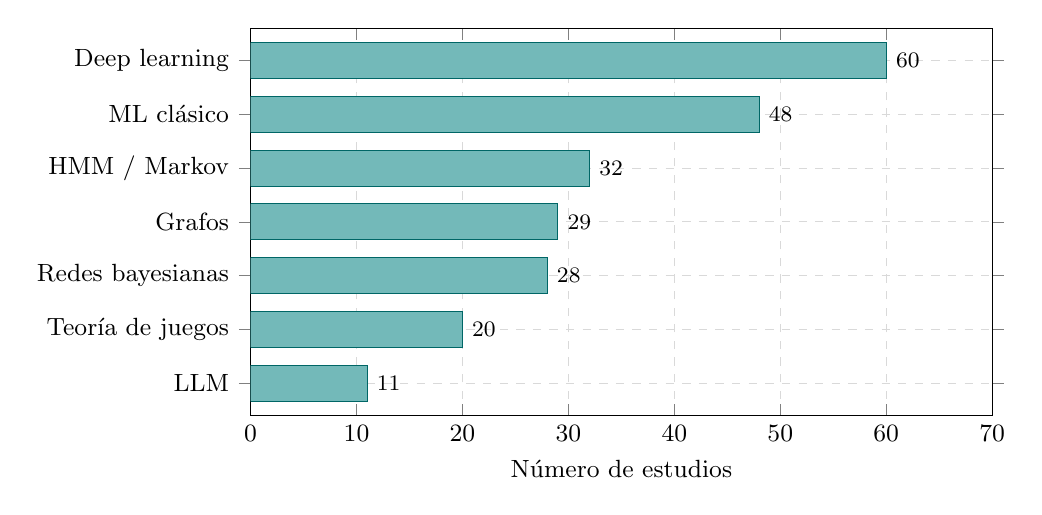
\begin{tikzpicture}
\begin{axis}[
    width=11cm, height=6.5cm,
    xbar, bar width=13pt,
    xmin=0, xmax=70,
    symbolic y coords={LLM,Teoría de juegos,Redes bayesianas,Grafos,HMM / Markov,ML clásico,Deep learning},
    ytick=data,
    xlabel={Número de estudios},
    nodes near coords, nodes near coords style={font=\footnotesize},
    grid=major, grid style={dashed,gray!30},
    tick label style={font=\small}, label style={font=\small},
]
\addplot[fill=teal!55,draw=teal!80!black] coordinates {(11,LLM)(20,Teoría de juegos)(28,Redes bayesianas)(29,Grafos)(32,HMM / Markov)(48,ML clásico)(60,Deep learning)};
\end{axis}
\end{tikzpicture}
\caption{Familias de modelos empleadas en los estudios del corpus. Fuente: Elaboración propia.}
\label{fig:modelos}
\end{figure}

\section{Hallazgos por categoría de análisis}

Esta sección presenta el análisis organizado según las categorías definidas en la metodología. La Tabla~\ref{tab:hallazgos} identifica, para cada estudio del corpus, las familias de modelos empleadas, los conjuntos de datos utilizados y el tratamiento explícito del desbalance de clases.

La revisión de los textos completos permite precisar la caracterización del corpus. Treinta y dos estudios mencionan modelos de Markov en alguna de sus variantes, de los cuales diecinueve refieren específicamente Modelos Ocultos de Markov. Nueve estudios trabajan con DAPT2020 y nueve con Unraveled, cifras superiores a las que sugería el análisis de resúmenes, lo que indica que una proporción relevante de los trabajos no declara el conjunto de datos en dicha sección. Treinta y seis estudios abordan de manera explícita el desbalance de clases, cerca de la mitad del corpus. Cabe precisar que estas cifras corresponden a la presencia de los términos en el texto completo, por lo que incluyen tanto el uso efectivo como las referencias a trabajos previos.

\begin{footnotesize}
\setlength{\tabcolsep}{4pt}
\renewcommand{\arraystretch}{1.15}
\begin{xltabular}{\linewidth}{|p{3.3cm}|c|X|p{3.6cm}|c|}

\caption{Hallazgos por categoría de análisis en los estudios del corpus}
\label{tab:hallazgos} \\
\hline
\textbf{Estudio} & \textbf{Año} & \textbf{Modelos / Técnicas} & \textbf{Conjuntos de datos} & \textbf{Desb.} \\
\hline
\endfirsthead

\caption[]{Hallazgos por categoría de análisis en los estudios del corpus (Continuación)} \\
\hline
\textbf{Estudio} & \textbf{Año} & \textbf{Modelos / Técnicas} & \textbf{Conjuntos de datos} & \textbf{Desb.} \\
\hline
\endhead

\hline
\multicolumn{5}{|r|}{\textit{Continúa en la siguiente página\dots}} \\ \hline
\endfoot

\hline
\endlastfoot


Açıkgözoğlu \parencite{acikgozoglu_explainable_2026}& 2026 & Deep L., ML clás., Juegos & ToN-IoT & x \\
Alsubait \parencite{alsubait_large_2026} & 2026 & Markov, Grafos, Deep L., LLM & CICIDS, NSL-KDD & x \\
El Alami et al. \parencite{el_alami_real-time_2026} & 2026 & Deep L., ML clás., LLM & CICIDS, UNSW, KDD99 & x \\
Ferazza et al. \parencite{ferazza_logs_2026} & 2026 & Deep L., LLM & -- & x \\
Giacobbe et al. \parencite{giacobbe_enforcing_2026} & 2026 & Markov & -- &  \\
Hölbl y Rotovnik \parencite{holbl_machine_2026} & 2026 & Bayes, Grafos, Deep L., ML clás. & DAPT2020, Unraveled, DARPA, CICAPT, CICIDS, NSL-KDD, UNSW & x \\
Hussain y Petrova \parencite{hussain_threat_2026} & 2026 & Bayes, Deep L., ML clás., LLM & -- & x \\
Jiao et al. \parencite{jiao_bg-flipin_2026} & 2026 & Markov, Bayes, Juegos & -- &  \\
K et al. \parencite{k_advanced_2026} & 2026 & Bayes, Grafos, Deep L., ML clás. & DAPT2020, Unraveled, CICAPT, NSL-KDD, UNSW, ToN-IoT, KDD99 & x \\
Kumar et al. \parencite{kumar_hlpmmgrsphtru_2026} & 2026 & HMM, Deep L., ML clás. & CICIDS & x \\
Lahari et al. \parencite{lahari_intelligent_2026} & 2026 & Deep L., ML clás. & -- & x \\
M. U. Basharat et al. \parencite{m_u_basharat_advanced_2026} & 2026 & Deep L., ML clás. & KDD99 & x \\
P. Firdani et al. \parencite{p_firdani_multi-layer_2026} & 2026 & Grafos, Deep L., LLM & DARPA, CICAPT & x \\
Puccetti et al. \parencite{puccetti_capture_2026} & 2026 & Grafos, Deep L., ML clás. & DAPT2020, Unraveled, DARPA, OpTC, CICAPT, CICIDS, NSL-KDD, ToN-IoT, KDD99 & x \\
R. Alfageer et al. \parencite{r_alfageer_multi-stage_2026} & 2026 & Deep L., ML clás., LLM & CICIDS, NSL-KDD, UNSW, ToN-IoT & x \\
R. Huang \parencite{r_huang_efficient_2026} & 2026 & Deep L., ML clás. & -- & x \\
Salah et al. \parencite{salah_dual-model_2026} & 2026 & Grafos, Deep L., ML clás., LLM & CICAPT, CICIDS, UNSW, ToN-IoT & x \\
Shahzad et al. \parencite{shahzad_autonomous_2026} & 2026 & Markov, Deep L., ML clás. & CICIDS, NSL-KDD, UNSW, ToN-IoT &  \\
Sripada et al. \parencite{sripada_hybridml_2026} & 2026 & Bayes, Deep L., ML clás., Juegos & CICIDS, NSL-KDD, UNSW, ToN-IoT, KDD99 & x \\
Yilmaz et al. \parencite{yilmaz_non-local_2026} & 2026 & Bayes, Deep L., ML clás. & CICIDS, UNSW, ToN-IoT & x \\
You et al. \parencite{you_comparative_2026} & 2026 & Deep L., ML clás. & CICIDS, NSL-KDD, UNSW & x \\
Zhao et al. \parencite{zhao_alert-driven_2026} & 2026 & Bayes, Deep L., Juegos & -- &  \\
Bani Melhem et al. \parencite{bani_melhem_lens_2025} & 2025 & Deep L., ML clás., LLM & CICAPT & x \\
Benabderrahmane et al. \parencite{benabderrahmane_ranking-enhanced_2025} & 2025 & Grafos, Deep L., ML clás. & DARPA, CICIDS, NSL-KDD, UNSW, KDD99 & x \\
Cai et al. \parencite{cai_detecting_2025} & 2025 & Bayes, Grafos, Deep L., ML clás. & Unraveled & x \\
Chen y Yan \parencite{chen_research_2025} & 2025 & Deep L., ML clás. & -- & x \\
Chourasiya et al. \parencite{chourasiya_advanced_2025} & 2025 & Bayes, Deep L., ML clás., LLM & CICIDS, UNSW &  \\
Ibrahim et al. \parencite{ibrahim_optimized_2025} & 2025 & Deep L., ML clás. & DAPT2020, Unraveled, CICIDS, NSL-KDD, UNSW &  \\
L. Zhang \parencite{l_zhang_implementing_2025} & 2025 & Deep L., ML clás. & DARPA & x \\
Mittal et al. \parencite{mittal_proactive_2025} & 2025 & HMM, Markov, Grafos, Deep L., ML clás., Juegos & -- & x \\
Nicho et al. \parencite{nicho_enhanced_2025} & 2025 & HMM, Bayes, Deep L., ML clás. & -- & x \\
Rivas et al. \parencite{rivas_analysis_2025} & 2025 & Bayes, Deep L., ML clás., Juegos & DAPT2020, Unraveled & x \\
S. Lee et al. \parencite{s_lee_aptstop_2025} & 2025 & HMM, Bayes, Grafos, Deep L., ML clás., LLM, Juegos & DARPA &  \\
Byrapuneni y Saidireddy \parencite{byrapuneni_efficient_2024} & 2024 & Bayes, Deep L., ML clás. & DARPA, NSL-KDD, KDD99 & x \\
Cheng et al. \parencite{cheng_kairos_2024} & 2024 & Grafos, Deep L. & DARPA, OpTC &  \\
Erfan Mazaheri y Shameli-Sendi \parencite{erfan_mazaheri_aptracker_2024} & 2024 & Bayes, Deep L., ML clás. & -- & x \\
J. Jiao et al. \parencite{j_jiao_fpgaa_2024} & 2024 & Grafos, Deep L. & DARPA &  \\
Lo et al. \parencite{lo_digital_2024} & 2024 & Deep L. & -- &  \\
Ma et al. \parencite{ma_anomaly_2024} & 2024 & HMM, Markov, Bayes, Deep L., ML clás. & DARPA, CICIDS &  \\
Mamun et al. \parencite{mamun_limitations_2024} & 2024 & Bayes, Deep L., ML clás. & DAPT2020, Unraveled, DARPA, CICIDS, NSL-KDD, UNSW, KDD99 & x \\
Soliman et al.\parencite{soliman_rank_2024}  & 2024 & Grafos, Deep L. & DARPA, KDD99 &  \\
Zhang et al. \parencite{zhang_secaas-based_2024} & 2024 & Markov, Grafos, Deep L., Juegos & -- &  \\
Chen et al. \parencite{chen_machine_2023} & 2023 & Deep L., ML clás. & CICIDS, NSL-KDD, UNSW, ToN-IoT, KDD99 & x \\
Javed et al. \parencite{javed_apt_2023} & 2023 & HMM, Bayes, Deep L., ML clás., LLM, Juegos & DAPT2020, CICIDS, NSL-KDD & x \\
Kazeminajafabadi y Imani \parencite{kazeminajafabadi_optimal_2023} & 2023 & HMM, Markov, Bayes, Grafos, Deep L. & -- &  \\
Kim et al. \parencite{kim_ban_2023} & 2023 & HMM, Markov, Bayes, Grafos, Deep L., Juegos & DAPT2020, Unraveled, DARPA &  \\
Kumari y Lee \parencite{kumari_prospective_2023} & 2023 & Markov, Deep L., ML clás. & DAPT2020, Unraveled & x \\
Smiliotopoulos et al. \parencite{smiliotopoulos_detection_2023} & 2023 & Bayes, Deep L., ML clás. & -- & x \\
Wan et al. \parencite{wan_resisting_2023} & 2023 & ML clás., Juegos & -- &  \\
Y. Javed et al. \parencite{y_javed_prism_2023} & 2023 & HMM, Markov, Grafos, Deep L. & -- &  \\
Zhang et al. \parencite{zhang_application_2023} & 2023 & Markov, Grafos & -- &  \\
Alsanad y Altuwaijri \parencite{alsanad_advanced_2022} & 2022 & Deep L., ML clás. & CICIDS & x \\
Anjum et al. \parencite{anjum2021anubis} & 2022 & Bayes, Grafos, Deep L., ML clás. & DARPA, OpTC & x \\
Choumanof et al. \parencite{choumanof_introducing_2022} & 2022 & Deep L. & DARPA, NSL-KDD, UNSW, ToN-IoT, KDD99 &  \\
Liu et al. \parencite{liu_new_2022} & 2022 & Grafos, Deep L., ML clás. & -- &  \\
Yao et al. \parencite{yao_intrusion_2022} & 2022 & Markov, Bayes, Deep L., Juegos & -- &  \\
Al Amin et al. \parencite{al_amin_hidden_2021} & 2021 & HMM, Markov, Bayes, Grafos, Juegos & DARPA &  \\
Baksi y Upadhyaya \parencite{baksi_decepticon_2021} & 2021 & HMM, Juegos & DARPA &  \\
C. D. Xuan \parencite{c_d_xuan_detecting_2021} & 2021 & Deep L., ML clás. & -- &  \\
Guillen et al. \parencite{guillen_propagation_2021} & 2021 & Markov, Bayes, Deep L., ML clás. & -- &  \\
Hoffmann \parencite{hoffmann_markov_2021} & 2021 & Markov & -- &  \\
Kim et al. \parencite{kim_intrusion_2021} & 2021 & Deep L., ML clás. & DARPA, NSL-KDD, UNSW, KDD99 &  \\
Min et al. \parencite{min_network_2021} & 2021 & Deep L., ML clás. & DARPA, CICIDS, NSL-KDD, UNSW, KDD99 & x \\
T. Shawly et al. \parencite{t_shawly_architectures_2021} & 2021 & HMM, Markov, Grafos, Deep L. & DARPA &  \\
Holgado et al. \parencite{holgado_real-time_2020} & 2020 & HMM, Markov, Bayes, Grafos & DARPA &  \\
L. Wang et al. \parencite{l_wang_method_2020} & 2020 & Bayes, ML clás. & -- &  \\
M. Khosravi y B. T. Ladani \parencite{m_khosravi_alerts_2020} & 2020 & HMM, Markov, Grafos & DARPA &  \\
A. Chowdhary et al. \parencite{a_chowdhary_adaptive_2019} & 2019 & Markov, Grafos, Juegos & -- &  \\
Brogi y Di Bernardino \parencite{brogi_hidden_2019} & 2019 & HMM, Markov, ML clás., Juegos & -- &  \\
Du et al. \parencite{du_attack_2019} & 2019 & HMM & -- &  \\
G. Ioannou et al. \parencite{g_ioannou_markov_2019} & 2019 & HMM, Markov, Bayes, Grafos, Juegos & -- &  \\
Ghafir et al. \parencite{ghafir2019hmm} & 2019 & HMM, Markov, Deep L., ML clás., Juegos & -- &  \\
Wang et al. \parencite{wang_optimal_2019} & 2019 & Markov, Deep L., Juegos & -- &  \\
Zegeye et al. \parencite{zegeye_multi-layer_2019} & 2019 & HMM, Markov, Deep L., ML clás. & CICIDS, NSL-KDD &  \\
D. Gonzales et al. \parencite{d_gonzales_cloud-trustsecurity_2017} & 2017 & Bayes, Grafos & -- &  \\
Niu et al. \parencite{niu_modeling_2017} & 2017 & Grafos & -- &  \\
Rass et al. \parencite{rass_defending_2017} & 2017 & Markov, Grafos, ML clás., Juegos & -- &  \\

\end{xltabular}
\end{footnotesize}

\section{Modelos probabilísticos aplicados a la detección de APT (RQ1)}

La evidencia recopilada muestra que los enfoques probabilísticos mantienen una presencia relevante en el área, pese al predominio reciente de los métodos basados en aprendizaje profundo. Los estudios identificados se agrupan en tres grandes líneas.

La primera corresponde a los modelos basados en redes bayesianas, empleados principalmente para representar dependencias entre eventos de seguridad y estimar la probabilidad de compromiso de distintos recursos de la red. Dentro de esta línea, \textcite{kazeminajafabadi_optimal_2023} modelan la red mediante grafos de ataque bayesianos para optimizar el monitoreo y la detección, mientras que \textcite{kim_ban_2023} integran el marco MITRE ATT\&CK en una red bayesiana para la predicción de campañas APT. Por su parte, \textcite{guillen_propagation_2021} emplean redes bayesianas dinámicas para modelar la propagación del malware utilizado en este tipo de campañas.

La segunda línea agrupa los enfoques basados en teoría de juegos, que modelan la interacción entre atacante y defensor como un proceso estratégico bajo incertidumbre \parencite{rass_defending_2017}. Trabajos posteriores extienden esta aproximación mediante hipergiegos para resistir múltiples campañas simultáneas \parencite{wan_resisting_2023} y mediante marcos bayesianos aplicados a modelos de amenaza interna \parencite{jiao_bg-flipin_2026}. Estas propuestas resultan de interés para el diseño de estrategias de defensa, aunque su orientación es prescriptiva más que detectiva: buscan determinar la respuesta óptima ante un adversario, antes que inferir el estado en que este se encuentra.

Una línea intermedia la constituyen los modelos de estado parcialmente observable, entre los que destacan el modelo multifase de creencia transferible de \textcite{g_ioannou_markov_2019} y la propuesta de \textcite{zhang_secaas-based_2024} para entornos industriales, que comparten con los HMM la premisa de que el estado del atacante no es directamente observable.

La tercera línea, y la más directamente vinculada a este trabajo, corresponde a los modelos secuenciales basados en cadenas de Markov, analizados en detalle en la sección siguiente.

Una observación transversal a las tres líneas es que los modelos probabilísticos tienden a aplicarse sobre representaciones previamente procesadas del comportamiento del atacante (alertas correlacionadas, grafos de ataque o indicadores de compromiso) antes que directamente sobre el tráfico de red. Esta dependencia de una etapa previa de procesamiento introduce un punto de falla adicional y condiciona el desempeño del modelo a la calidad de dicha correlación.

\section{Modelos Ocultos de Markov aplicados a APT (RQ2)}

De los 32 estudios que mencionan modelos de Markov, diecinueve aplican específicamente Modelos Ocultos de Markov a la detección o predicción de campañas APT, lo que confirma la pertinencia del enfoque adoptado en este trabajo y proporciona una base comparativa para su evaluación.

El precedente metodológico más directo corresponde al trabajo de \textcite{ghafir2019hmm}, que emplea un HMM para determinar la secuencia más probable de etapas de una APT a partir de alertas correlacionadas, incorporando un algoritmo de predicción del siguiente paso del atacante. En una línea similar, \textcite{holgado_real-time_2020} proponen un sistema de predicción de ataques multi-etapa en tiempo real basado en HMM, evaluado sobre alertas provenientes de sistemas de detección de intrusiones, mientras que \textcite{brogi_hidden_2019} modelan la evolución de una campaña APT como un proceso de Markov oculto sobre observaciones de red. \textcite{du_attack_2019} abordan específicamente la predicción de la ruta de ataque mediante HMM.

Otras propuestas exploran variantes arquitectónicas del modelo. \textcite{zegeye_multi-layer_2019} proponen un sistema de detección de intrusiones basado en HMM multicapa, y \textcite{t_shawly_architectures_2021} analizan arquitecturas orientadas a la detección de ataques multi-etapa entrelazados, escenario en que múltiples campañas se solapan temporalmente. Complementariamente, \textcite{baksi_decepticon_2021} proponen Decepticon, un framework basado en HMM que utiliza indicadores de compromiso como variables observables, orientado a contrarrestar campañas APT mediante mecanismos de engaño, enfoque que \textcite{al_amin_hidden_2021} extienden combinando HMM y decepción para la prevención de movimientos adversariales. Por su parte, \textcite{hoffmann_markov_2021} modelan el ciclo de vida completo del ataque como un proceso de Markov desencadenado por vulnerabilidades de software.

El análisis de estos trabajos permite identificar un patrón común en la definición del modelo: los estados ocultos se corresponden con las etapas de la cadena de ataque, mientras que las variables observables se derivan de alertas o indicadores previamente generados por otros sistemas. Esta decisión de diseño, si bien reduce la dimensionalidad del espacio de observaciones, hace que el modelo dependa de una infraestructura de detección previa y limita su aplicabilidad en escenarios donde dicha infraestructura no está disponible o produce alertas incompletas.

\section{Conjuntos de datos utilizados (RQ3)}

La Figura~\ref{fig:datasets} presenta los conjuntos de datos mencionados en el texto completo de los estudios del corpus. El hallazgo más relevante de esta dimensión es la ausencia de un conjunto de referencia consolidado: la categoría más frecuente, con 33 estudios, corresponde a trabajos que no declaran un conjunto público (conjuntos propios, generados sintéticamente o propuestas sin evaluación sobre datos abiertos), y ningún conjunto público alcanza un tercio del corpus. Entre los públicos predominan DARPA/OpTC y conjuntos de intrusiones de uso general (CICIDS, NSL-KDD, UNSW-NB15, KDD99), mientras que los conjuntos etiquetados por etapas de APT, DAPT2020 y Unraveled, aparecen en nueve estudios cada uno, lo que dificulta la comparación directa entre propuestas.

\begin{figure}[h!]
\centering
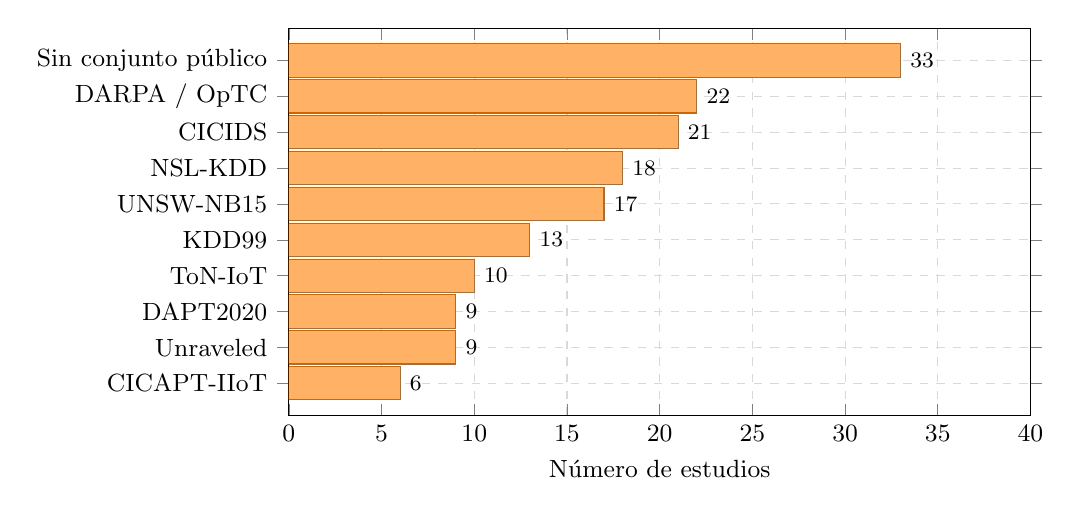
\begin{tikzpicture}
\begin{axis}[
    width=11cm, height=6.5cm,
    xbar, bar width=12pt,
    xmin=0, xmax=40,
    symbolic y coords={CICAPT-IIoT,Unraveled,DAPT2020,ToN-IoT,KDD99,UNSW-NB15,NSL-KDD,CICIDS,{DARPA / OpTC},{Sin conjunto público}},
    ytick=data,
    xlabel={Número de estudios},
    nodes near coords, nodes near coords style={font=\footnotesize},
    grid=major, grid style={dashed,gray!30},
    tick label style={font=\small}, label style={font=\small},
]
\addplot[fill=orange!60,draw=orange!80!black] coordinates {(6,CICAPT-IIoT)(9,Unraveled)(9,DAPT2020)(10,ToN-IoT)(13,KDD99)(17,UNSW-NB15)(18,NSL-KDD)(21,CICIDS)(22,{DARPA / OpTC})(33,{Sin conjunto público})};
\end{axis}
\end{tikzpicture}
\caption{Conjuntos de datos mencionados en los estudios del corpus. Fuente: Elaboración propia.}
\label{fig:datasets}
\end{figure}
\FloatBarrier

Entre los conjuntos con etiquetado por etapas de ataque, DAPT2020 \parencite{myneni2020dapt2020} y Unraveled \parencite{myneni2023unraveled} son los que presentan mayor correspondencia con los requerimientos de un modelo secuencial, dado que su estructura identifica explícitamente la fase de la campaña a la que corresponde cada registro. Ambos conjuntos han sido empleados conjuntamente en trabajos recientes de detección de APT \parencite{rivas_analysis_2025}. Los conjuntos de intrusiones de uso general, como NSL-KDD, CICIDS o UNSW-NB15, carecen de este etiquetado y presentan una separación entre tráfico legítimo y malicioso que no refleja la sofisticación de un adversario APT.

La literatura reciente documenta de forma explícita estas limitaciones. \textcite{mamun_limitations_2024} analizan sistemáticamente los conjuntos de datos disponibles para investigación en APT y concluyen que tienden a cubrir periodos breves, a subrepresentar las etapas intermedias de la campaña y a presentar distribuciones de clase que no reproducen las condiciones de operación reales. Esta constatación ha motivado la aparición de nuevos conjuntos orientados a corregir dichas carencias, entre ellos el benchmark propuesto por \textcite{liu_new_2022}, el conjunto CYSAS-S3 \parencite{choumanof_introducing_2022}, el conjunto de malware con atribución a grupos APT de \textcite{erfan_mazaheri_aptracker_2024} y, más recientemente, el conjunto cAPTure \parencite{puccetti_capture_2026}, orientado específicamente a evaluar la rapidez de detección. La persistencia de esta línea de trabajo confirma que la disponibilidad de datos representativos constituye un problema abierto en el área, y fundamenta la decisión de emplear dos conjuntos complementarios en el presente trabajo.

\section{Estrategias frente al desbalance de clases (RQ4)}

Treinta y seis estudios del corpus abordan explícitamente el problema del desbalance de clases en la detección de amenazas, cerca de la mitad del total. Las estrategias identificadas se concentran en técnicas de remuestreo, entre las que predomina el sobremuestreo sintético de la clase minoritaria \parencite{chawla2002smote}, junto con aproximaciones híbridas que combinan sobremuestreo y submuestreo. Estas técnicas operan sobre instancias tratadas como independientes entre sí, supuesto cuyas implicancias para un modelo secuencial se discuten en el Capítulo~\ref{cap:propuesta}.

No obstante, el hallazgo más significativo de esta dimensión no proviene de las estrategias empleadas, sino de las métricas utilizadas para evaluarlas. Como muestra la Figura~\ref{fig:metricas}, 35 estudios del corpus reportan \textit{accuracy}, mientras que solo 14 reportan F1-score, 8 precisión y 6 exhaustividad. Esta distribución resulta problemática: en escenarios con desbalance severo, donde la actividad maliciosa constituye una fracción mínima del tráfico total, la exactitud global puede alcanzar valores elevados aun cuando el modelo falle sistemáticamente en la clase minoritaria, que es precisamente la de interés.

\begin{figure}[h!]
\centering
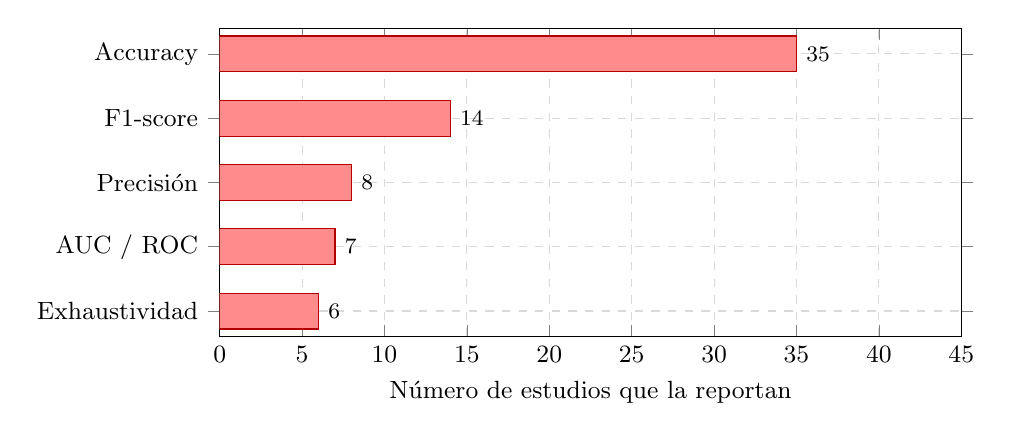
\begin{tikzpicture}
\begin{axis}[
    width=11cm, height=5.5cm,
    xbar, bar width=13pt,
    xmin=0, xmax=45,
    symbolic y coords={Exhaustividad,{AUC / ROC},Precisión,F1-score,Accuracy},
    ytick=data,
    xlabel={Número de estudios que la reportan},
    nodes near coords, nodes near coords style={font=\footnotesize},
    grid=major, grid style={dashed,gray!30},
    tick label style={font=\small}, label style={font=\small},
]
\addplot[fill=red!45,draw=red!70!black] coordinates {(6,Exhaustividad)(7,{AUC / ROC})(8,Precisión)(14,F1-score)(35,Accuracy)};
\end{axis}
\end{tikzpicture}
\caption{Métricas de evaluación reportadas en los estudios del corpus. Fuente: Elaboración propia.}
\label{fig:metricas}
\end{figure}
\FloatBarrier

En consecuencia, una proporción considerable de la literatura evalúa sus propuestas mediante una métrica que enmascara el problema que declara abordar, y son minoría los trabajos que reportan el desempeño de forma desagregada por clase o por etapa de ataque.

\section{Síntesis y brechas identificadas}

El análisis del corpus permite identificar cuatro brechas que fundamentan la propuesta de este trabajo.

\begin{itemize}
    \item En primer lugar, los modelos probabilísticos aplicados a la detección de APT operan mayoritariamente sobre alertas o indicadores previamente correlacionados, lo que introduce una dependencia respecto de una infraestructura de detección previa.
    \item En segundo lugar, si bien los Modelos Ocultos de Markov cuentan con precedentes consolidados en el dominio, su aplicación directa sobre tráfico de red etiquetado por etapas de ataque se encuentra escasamente explorada.
    \item En tercer lugar, no existe un conjunto de datos de referencia consolidado para la evaluación de propuestas en el área, y los conjuntos con etiquetado por etapas presentan una adopción limitada pese a ser los más adecuados para enfoques secuenciales.
    \item En cuarto lugar, y de manera transversal, la literatura evalúa predominantemente mediante métricas globales que no permiten observar el desempeño sobre la clase minoritaria, lo que impide determinar si las propuestas existentes mantienen su efectividad bajo las condiciones de desbalance que caracterizan a los escenarios reales.
\end{itemize}

Estas cuatro brechas configuran el espacio de oportunidad que aborda la propuesta descrita en el capítulo siguiente.